\documentclass[12 pt]{report}

\usepackage{epsfig}
\usepackage[in,empty]{myfullpage}
\usepackage{amssymb}
\usepackage{amsmath}

\baselineskip=20pt

\begin{document}

\noindent \vfill \noindent \large

\centerline{Math 324 C  - Summer 2016}

\centerline{Midterm exam 1}

\centerline{Wednesday, July 13th, 2016}

\normalsize

\vfill
\medskip
Name: \rule{10cm}{1pt}

\bigskip

\vfill
\begin{center}
{\large
\begin{tabular}{||c|c|r||}
\hline Problem 1 & 10 & \hspace{10mm} \hfill \\
\hline Problem 2 & 10  & \hspace{10mm} \hfill \\
\hline Problem 3 & 10 & \hspace{10mm} \hfill \\
\hline Problem 4 & 10  & \hspace{10mm} \hfill \\
\hline Problem 5 & 10  & \hspace{10mm} \hfill \\
\hline Total & 50 & \hspace{10mm} \hfill \\
\hline
\end{tabular}
}
\end{center}
\vfill
\begin{itemize}
\item There are 5 questions on this exam. Make sure you have all five.
\item You must show your work on all problems.  The correct answer
with no supporting work may result in no credit. \textbf{Put a box
around your FINAL ANSWER for each problem and cross out any work
that you don't want to be graded.} 
\item Give exact answers, and simplify as much as possible. 
For example, $\frac{\pi}{\sqrt{2}}$ is acceptable, but $\frac{1}{2} + \frac{3}{4}$
should be simplified to $\frac{5}{4}$.  

\item If you need more room, use the backs
of the pages and indicate to the grader that you have done so.
\item Raise your hand if you have a question.
\item Any student found engaging in academic misconduct will receive
a score of 0 on this exam.
\item You have 60 minutes to complete the exam.  Budget your time wisely! \\
\end{itemize}
\vfill
\begin{center}GOOD LUCK!\end{center}

\newpage
\begin{enumerate}

\item (10 pts) Recall that the \textbf{average value} of a function $f:[a,b] \to \mathbb{R}$ is given by

$$\frac{1}{b-a} \int_a^b f(x) \, dx.$$

Similarly, for a function $f:R \to \mathbb{R}$ on a 2D-region $R$, the average value is given by

$$\frac{1}{\text{area}(R)} \iint_R f \, dA,$$

and for a function $f:E \to \mathbb{R}$ on a 3D-region $E$, the average value is

$$\frac{1}{\text{vol}(E)} \iiint_E f \, dV.$$

\begin{enumerate} \item[a.] Find the average value of $f(x) = x^2$ over the interval $[-1,1]$. 

\item[b.] Find the average value of $f(r,\theta) = r^2$ over the unit disk 
$$\{(r,\theta): 0 \leq \theta \leq 2\pi, 0 \leq r \leq 1\}.$$ 

\item[c.] Find the average value of $f(\rho, \theta, \phi) = \rho^2$ over the unit sphere 
$$\{(\rho, \theta, \phi): 0 \leq \theta \leq 2\pi, 0 \leq \phi \leq \pi, 0 \leq \rho \leq 1\}.$$ 

\end{enumerate} \vfill

\newpage

\item (10 pts) Let $R$ be the region in the plane given by 

$$R = \{(r, \theta): \frac{1}{2} \csc \theta \leq r \leq \sin \theta, 0 \leq r < \infty, 0 \leq \theta \leq \pi\}.$$

Sketch the region $R$, and evaluate the double integral 

$$\iint_R \sin^2\theta \, dA.$$ 

\newpage

\item (10 pts) Use the change of coordinates $x = u-2v, y = v$ to set up the integral 

$$\iint_R (x+3y) \, dA$$

in $u,v$ coordinates, where $R$ is the region in the $x-y$ plane bounded by the curves 
$$y=1, y=3, x+2y=10, x+2y=6.$$

The region $R$ is pictured below. Sketch the image region after changing coordinates, and explain how you know what the new region looks like. \textbf{You do not need to evaluate the integral.}

\flushleft 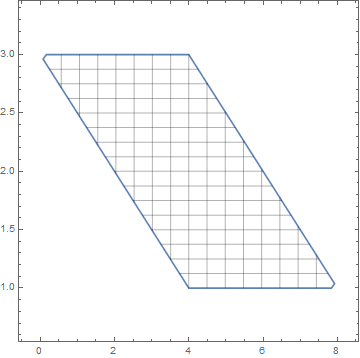
\includegraphics[width=3in]{midterm1_problem_3.png}


\newpage

\item[4.] (10 pts) Set up but \textbf{do not evaluate} the integral 
$$\iiint_E xz \, dV$$

in Cartesian coordinates, where $E$ is the solid (with finite volume) that is bounded by the surfaces 

$$x=y^4, x=2y^2-1, z = 0 \text{ and } z=3y.$$

(For example, ``the surface $x=y^4$" means the set of all points $(x,y,z) \in \mathbb{R}^3$ satisfying $x=y^4$.)
\newpage

\item[5.] (10 pts) Professor Stella Artois wants to know how much beer her strangely shaped beer bottle can hold. The design is obtained by rotating the curve $x = 2+\cos \pi z, 0 \leq z \leq 5$ (in the $x-z$ plane) around the $z$ axis, and attaching caps at the top and bottom. Beer tends to be foamier at the top: the density of beer in the bottle is 

$$d(x, y, z) = \frac{6-z}{1+\frac{1}{2}\cos \pi z}.$$

(The $1+\frac{1}{2}\cos \pi z$ is the so called `sloshing term,' to account for the movement of the beer inside the bottle.) Compute the mass of the beer in the bottle when it is full, by integrating the function $d$ over the the region occupied by the bottle. 




\end{enumerate}

\end{document}
